\subsection{Alternating Bit Protocol - Tool Usage Example}
In this section we present how to use the tool to show that the specification and 
implementation of the ABP are weakly bisimiliar. As a first step we always need to
generate the LTSs from both the specification and implementation of the system that
we are trying to model. That can be done in the tab "CCS to LTS" in the tool. As shown
in \ref{fig:abptoolusage1} in the upper text area we need to write down the ccs 
expressions that describe the system or load them from a file. One constraint here
is that a general ccs expression that describes the whole system has to be put on
the first line. The algorithm for generating the LTS graph starts evaulation and 
construction of the graph starting from the first line. When we have our ccs expressions
put in place we have to click "Generate LTS". This action will make the application
parse the expression and if no errors are found will start generating the LTS graph
The results from the generated graph will be presented in the lower text area in 
Aldebaran format. The users can save the results in a file or can click "View LTS Graph" 
which causes the tool to display a computer generated image of the LTS graph.

LTS minimization can be done in the "LTS minimization" tab. The minimization is pretty 
straigthforward process. As shown in \ref{fig:abptoolusage2} and \ref{fig:abptoolusage3}
LTS is loaded from file, a method of calculation has to be chosen and in order to perform
calculation the user has to click the button "Calculate".

Checking for LTS bisimilarity is performed in the "LTS comparison" tab. This tab is 
similary to the one for the minimization. As shown in \ref{fig:abptoolusage4} and
\ref{fig:abptoolusage5} two LTSs have to loaded from file. In order to check for LTS 
bisimilarity the user has to chose a method for calculatino and click on the button 
"Calculate". The results will be displayed on the right side of the button and they
give information wheather the LTSs are bisimilar and how long the calculation lasted.

\begin{figure}[!ht]
\centering
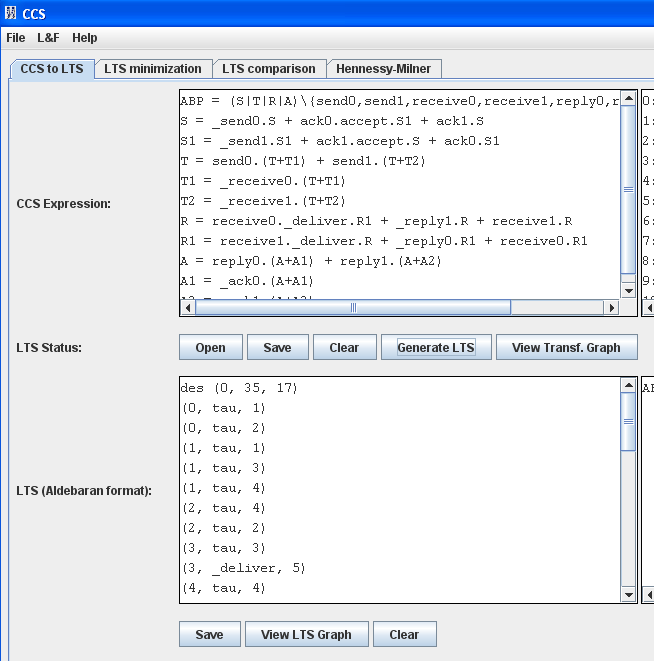
\includegraphics[width=5in]{ABPToolUsage1}
\caption{Tool Usage: ABP Modeling and Generating LTS}
\label{fig:abptoolusage1}
\end{figure}

\begin{figure}[!ht]
\centering
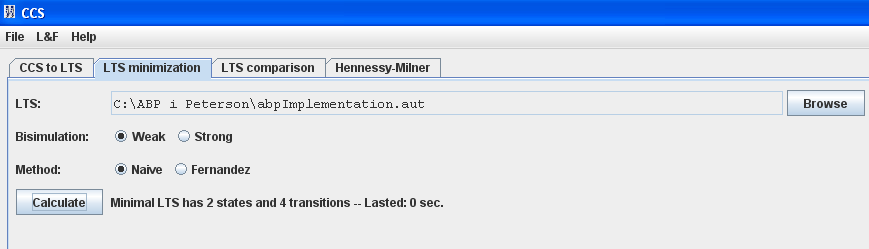
\includegraphics[width=5in]{ABPToolUsage2}
\caption{Tool Usage: ABP Minimization, Weak, Naive}
\label{fig:abptoolusage2}
\end{figure}

\begin{figure}[!ht]
\centering
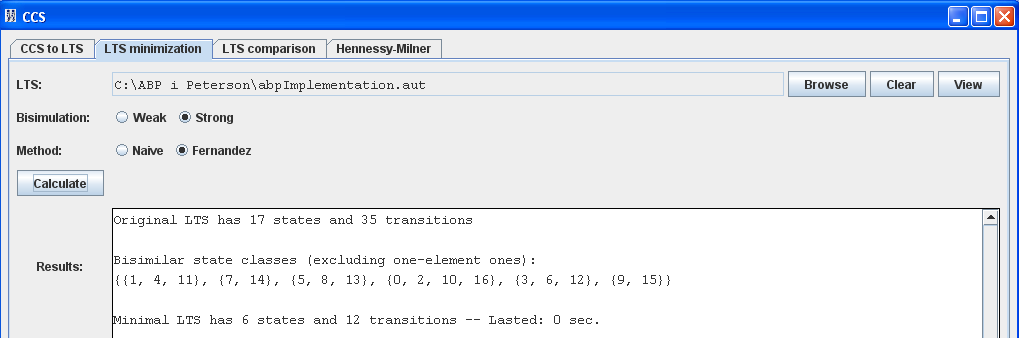
\includegraphics[width=5in]{ABPToolUsage3}
\caption{Tool Usage: ABP Minimization, Strong, Fernandez}
\label{fig:abptoolusage3}
\end{figure}

\begin{figure}[!ht]
\centering
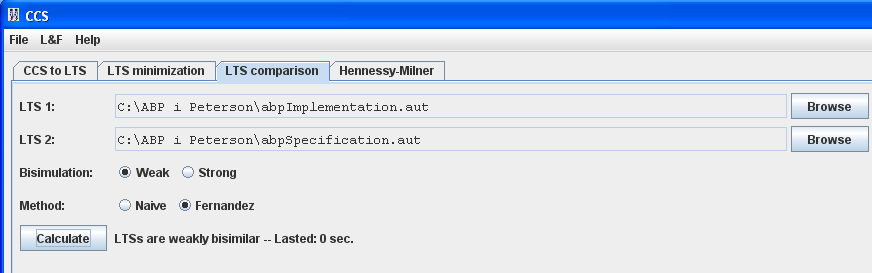
\includegraphics[width=5in]{ABPToolUsage4}
\caption{Tool Usage: ABP Bisimilarity, Weak, Fernandez}
\label{fig:abptoolusage4}
\end{figure}

\begin{figure}[!ht]
\centering
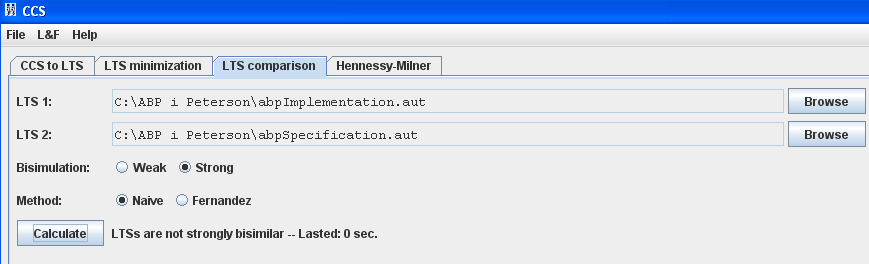
\includegraphics[width=5in]{ABPToolUsage5}
\caption{Tool Usage: ABP Bisimilarity, String, Naive}
\label{fig:abptoolusage5}
\end{figure}